% Todo:

\documentclass[12pt]{article}
\usepackage{hyperref}
\usepackage{xeCJK}
\usepackage{fontspec}
%\setCJKmainfont{SimSun}
\setCJKmainfont[BoldFont=SimHei,ItalicFont=KaiTi]{SimSun}
% \setCJKsansfont{SimHei}
% \setCJKmonofont{SimKai}
% \setmainfont{Arial}

\usepackage{cite}
\usepackage{graphicx}
\usepackage{float}
\usepackage{amsfonts}
% \usepackage{amsmath}	% for \tag
\usepackage{amssymb}	% for \multimap
% \usepackage{stmaryrd}
\usepackage{color}
%\usepackage[square,numbers]{natbib}
%\nocopyright
%\usepackage{latexsym,amsmath,amssymb,graphicx,hyperref}
%\usepackage{times} % gives you a bit more space if needed
\usepackage{titlesec}		% change color of section headings
\usepackage{verbatim}
\usepackage[most]{tcolorbox}		% color box

\makeatletter
\newsavebox{\@brx}
\newcommand{\llangle}[1][]{\savebox{\@brx}{\(\m@th{#1\langle}\)}%
  \mathopen{\copy\@brx\kern-0.5\wd\@brx\usebox{\@brx}}}
\newcommand{\rrangle}[1][]{\savebox{\@brx}{\(\m@th{#1\rangle}\)}%
  \mathclose{\copy\@brx\kern-0.5\wd\@brx\usebox{\@brx}}}
\makeatother

\titleformat{\section}
{\color{blue}\normalfont\Large\bfseries}
{\color{blue}\thesection}{1em}{}
\titleformat{\subsection}
{\color{blue}\normalfont\large\bfseries}
{\color{blue}\thesubsection}{1em}{}

\renewcommand\abstractname{\textcolor{blue}{Abstract}}

\definecolor{LogicColor}{rgb}{0.4,0.1,0.4}  % Magenta
\definecolor{Hilight}{rgb}{0.9,0.9,0.8}  % Magenta
% \definecolor{LogicColor}{rgb}{0,0,0}	% for black-and-white paper

\newcommand{\concept}[1]{\textbf{\textcolor{blue}{#1}}}

\newcommand{\english}[1]{\rmfamily \textit{``#1''}\rmfamily}
\newcommand{\formula}[1]{\textcolor{LogicColor}{#1}}

\newcommand{\hilight}[1]{\begin{tcolorbox}[breakable]#1\end{tcolorbox}}

\newcommand{\tab}{\hspace*{1cm}}

\newcommand{\df}{f} %probability density function
\newcommand{\dfo}{f1} %other probability density function
\newcommand{\fv}{x} %fuzzy variable
\newcommand{\zand}{\; \tilde{\wedge} \;}
\newcommand{\zor}{\; \tilde{\vee} \;}
\newcommand{\PimpL}{\leftarrowtriangle}
\newcommand{\com}{\multimap}
\newcommand{\comL}{\circ \hspace{-0.4em} - \,}
\newcommand{\mul}{}
\newcommand{\loves}{loves }
\newcommand{\heart}{\, \heartsuit \,}

\newcommand*\sigmoid{\vcenter{\hbox{
\includegraphics{sigmoid.png}}}}
\newcommand*\sadface{
\includegraphics[scale=0.25]{face-sad.png}}

\setlength{\oddsidemargin}{1cm}
\setlength{\evensidemargin}{1cm}
\setlength{\textwidth}{14cm}

\linespread{1.2}

\title{\textcolor{blue}{Genifer 4.1 理论笔记}}
\author{YKY (\textit{甄景贤})}
\date{30 June 2015}
% \institute{}

\begin{document}

\tab\tab\tab \parbox{9cm}{\textit{No problem can withstand the assault of sustained thinking.}}
% \vspace{-0.5cm}
\begin{flushright}
\textemdash\, Voltaire \hspace*{2cm}
\end{flushright}

\sffamily

{\let\newpage\relax\maketitle}

\maketitle
\setlength{\parindent}{0em}
\setlength{\parskip}{1.5ex plus0.5ex minus1.2ex}

现在来 recap 一下,我想做的是什么...

首先,我们有一个原子概念的集合 $A = \{ \mbox{男人}, \mbox{女人}, \mbox{爱}, \mbox{恨}, \mbox{足球},... \}$,在抽象代数中这个集通常叫作 alphabet,它的元素叫字母 (letters)。 

2013 年,Tom\'{a}\v{s} Mikolov 等人在 Google 研究出 Word2Vec,引起了广泛影响。  基本上它将离散的词汇集合映射到连续的向量空间(需要某种近似),这个近似是基於所谓的分布性原理 (Distributional Hypothesis),即是说: 两个词如果分布相似,即经常出现在相似的句子中,它们的语义也会相近。 

我们的目的不是探讨如何计算词汇的 distributive representation,而是假设在原始概念的层次上,这份工作已经做好,不管是用 Word2Vec 或其他的方法。  

% 给定一个字 $w$,Word2Vec 计算它最有可能的上下文 $c$,而 $c$ 是用参数 $\theta$ 给出的:
% $$ \arg \max_\theta \prod_{(w,c) \in D} p(c|w; \theta) $$

我们要处理的问题是: 由\textbf{词语}过渡到\textbf{句子},进而从事\textbf{推理}和\textbf{学习}。

表达句子的方法:
\begin{itemize}
\item 最简单可以只是 3 个元素构成的 $a \, R \, b$。
\item Smolensky 提出的 tensor 方法,可以表达任何树状结构。
\item 最新的研究方向,人们发现句子的结构和抽象代数的结构是一样的,所以注意力转移到抽象的範畴的研究,例如这本书:
\begin{figure}[H]
\centering
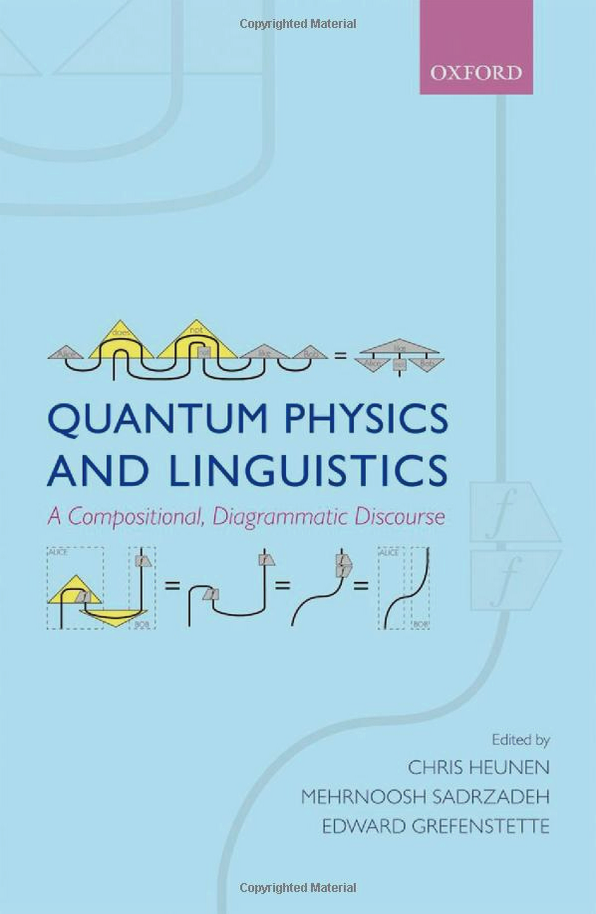
\includegraphics[scale=0.3]{quantum-physics-and-linguistics-book-cover.png}
\end{figure}
\end{itemize}

其中最一般的範畴是 monoidal categories,或者叫 tensor categories。  在向量空间里的 tensor product 是这个範畴中的一个例子。  换句话说,我们基本上是用 tensor product 来表达句子; 範畴论只是将这一点说得更一般化和抽象化而已。

\section{命题空间的 dimension}

在知识空间中,如果 $v_1, v_2, v_3$ 是三个互不相关的命题,那么它们的线性相关 $ a_1 v_1 + a_2 v_2 = a_3 v_3 $ 是不容许的,否则会出现谬误。 结论是: 要么知识空间的 dimension 等於命题的总数(那会很大,可能无限大),要么放弃 $a_i$ 是真假值的做法。

人的词汇 (vocabulary) 的个数大约在 3,000 至 10,000's 之间。  暂时假设我们可以用 dimensionality reduction 把原始概念的个数缩小到 3000,那么概念空间 $C$ 的维数就是 3000。

\hilight{
如果只考虑像 $a\, R\, b$ 那样的关系,则命题空间是 $C \times C \times C$,维数是 $3000 \times 3 = 9K $。 但如果是 $ C \otimes C \otimes C $ 则维数是 $ 3000^3 = 9G $。 现时的电脑记忆(例如 GPU)似乎可以处理后者。
}

\section{Distributive representation (分布式表示法)}

如果每个概念是向量空间中的一个独立分量,似乎很浪费空间。  在神经网络中通常用\textbf{分布式}的表示法:
\begin{figure}[H]
\centering
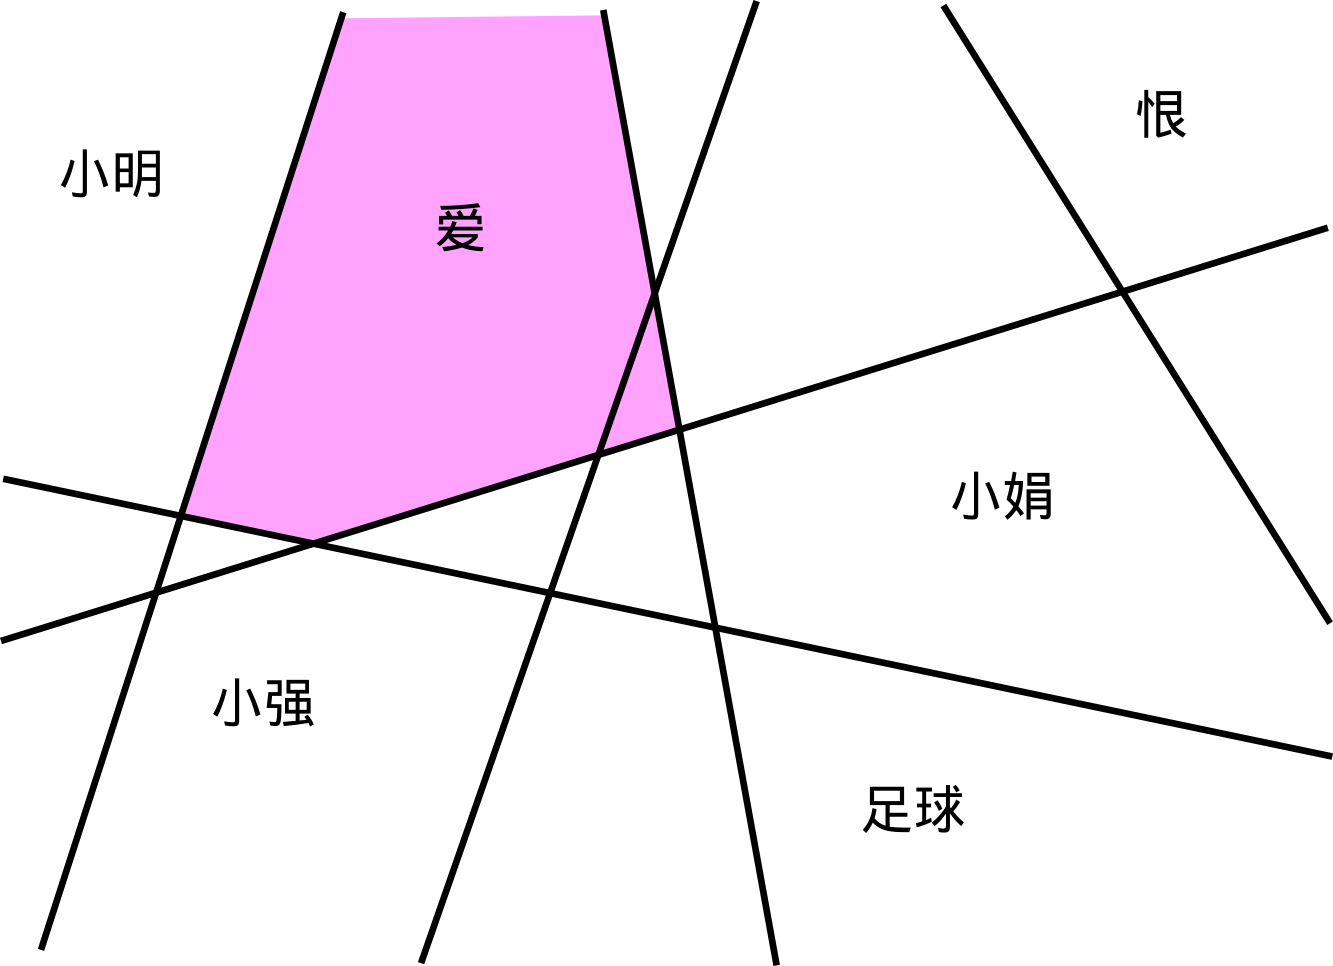
\includegraphics[scale=0.5]{distributive-vector-representation-linear.png}
\end{figure}

一粒神经元的公式是:  $y = \sigmoid (w^T x \leq b) $

(但如果只有一层神经元)那非线性函数可以不理(它不影响 decision boundary)。

$ (w^T x \leq b) $ 表示一个 hyperplane 的切割。

一个概念就是一组 hyperplanes 切割而成的多面体 (polyhedron),\\
\tab \tab $c : (Wx \leq B) $。\\
矩阵 $W$ 对应於一层神经网络中的 weights。

问题: 在这个表示法中,「线性无关」代表什么?

\section{「连续性」}

第二个问题是「连续」指的是什么。 例如命题 $P_1$ =「小明爱小娟」,$P_2$ =「小强爱踢足球」,那么由 $P_1$ 变化到 $P_2$ 必然会有 discrete jump,那是无可置疑的。 除非我们重新定义命题是像 $k_1 P_1+ k_2 P_2$ 那样的东西,才可以有「连续变化」;  这一点需要再加以精确化。

我发觉「连续空间」不是一个严谨的术语,因为在 discrete 空间中也可以定义 "continuous" 这概念,例如在 computer science 的 functional programming 里有 domain theory、 denotational semantics 等,常常谈到离散空间中的连续函数。 而且「可微分」的概念也有一些 generalizations,例如 Fr\'{e}chet derivatives(在泛函空间中)。

有个方法可以表示我想说的「连续空间」的性质: 在两点 $x \neq y$ 之间,总可以找到第三点 $z$,位置介乎 $x$ 与 $y$ 之间,换句话说:
$$ d(x,z) < d(x,y) \wedge d(y,z) < d(x,y). $$

似乎 Hausdoff 性质就是我想说的「连续空间」的性质: A Hausdorff space is a topological space in which distinct points have disjoint neighbourhoods.  

\section{近似}

那些算子或许可以合写成一个:
$$ T_1 v + T_2 v + ... + T_n v = \mathcal{T} v $$
然后合写后用 function approximation 来近似。

但这种近似必须有代价,否则违反了两项原则:
\begin{enumerate}
\item Turing 已经很有远见地意识到,逻辑推导的普适算法是不存在的,因为它违反了停机原理 (halting problem)。 后者是用 Cantor 的集合论中的 diagonal argument 证明的。 如果我们的优化算法必然会给出答案,而答案又可以转换回逻辑,那是不可能的。 所以在近似过程中必然会有某些误差。
\item 如果 $P \neq NP$,我们的算法也不可能总是在 polynomial time 之内回覆正确答案。
\end{enumerate}

\section{``Second-order''}

还有一个 "second-order" 的想法。  在 first-order 我们的算子是这个形式:
$$ T: V \rightarrow V $$  
但 second-order 的做法是将所有\textbf{物体}都看成是算子,算子可以作用在算子之上,这似乎是一种 duality。 

如果我们简单地将 $\mathcal{T}$ 近似,那些逻辑推导就会有错误。  或者应用某个 duality 或二次形式后,近似的做法会有较好结果?

从另一个角度看,详细一点分析那\textbf{推导}和\textbf{学习}的过程。  推导的过程是:
\begin{figure}[H]
\centering
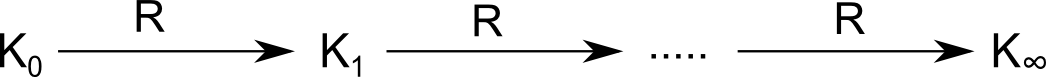
\includegraphics[scale=0.6]{2nd-order-maps-0.png}
\end{figure}
可以将它简写,并加上反向的 $L$ map:
\begin{figure}[H]
\centering
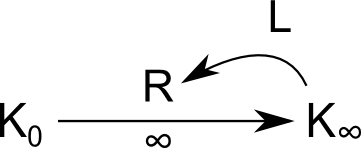
\includegraphics[scale=0.6]{2nd-order-maps-1.png}
\end{figure}
$L$ 是由结论 $K_\infty$ 到法则 $R$ 的映射,可以叫 $L$ 做 learning map。  这个 map 比较复杂,它相当於学习的过程,通常要用 iteration 逼近。  而且,有无限多个 $R$ 可以符合条件,我们通常选取长度短的 $R$,这是 minimum description length 原理,又或者选取资讯\textbf{压缩比}最高者。

上面的 map 可以再简化,因为 $K_0$ 是常项,可以省略。  写成垂直形式:
\begin{figure}[H]
\centering
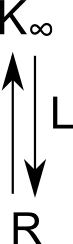
\includegraphics[scale=0.6]{2nd-order-maps-2.png}
\end{figure}

现在如果我们改变推导的结果 $K^*$,亦即改变 $K_\infty$,那么 $R$ 亦要改变成 $R'$,但 $L$ 未必要改变。  学习这个 $L$ 是一种\textbf{二次形式}的学习。
\begin{figure}[H]
\centering
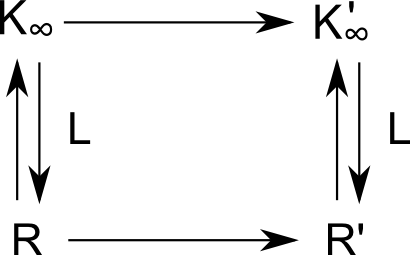
\includegraphics[scale=0.6]{2nd-order-maps-3.png}
\end{figure}

问题是 $R$ 的空间太大... 但 $R$ 是所有有意识的知识... 不想直接近似 $R$,但如何间接地近似它?  

\section{Metric 从何而来?}

現在概括一下\textbf{逻辑系统}是什么。  $\mathcal{L} = \{ C, P, +, \rightarrow, d(\cdot,\cdot), \subseteq \}$ 包含以下元素:
\begin{enumerate}
\item 原子概念集 $C \ni c_1, c_2, ...$
\item 命题集 $P \ni p_1, p_2, ...$ (可以限制在简单关系 $a\, R\, b$)
\item 连结词 (conjunction) $p_1 \wedge p_2$ 或 $p_1 + p_2$
\item 箭头 $p_1 + p_2 + ... \rightarrow p_0$
\item 概念之间的距离 $d(c_1, c_2)$
\item 概念之间的偏序 (partial order) $c_1 \subseteq c_2$
\end{enumerate}

但其实 $d(\cdot, \cdot)$ 和 $\subseteq$ 并不是逻辑\textbf{内在}的,它们是从资料中 induce 出来的。 其原理是基於 Liebniz extensionality:
$$ f = g \quad \Leftrightarrow \quad \forall x. \; f(x) = g(x). $$
它原本是描述两个函数的相等,但我们可以将它普及到任何概念的乘积:
$$ c_1 \approx c_2 \quad \Leftrightarrow \quad \forall_\# P, P'. \; P[c_1], P'[c_2]. $$
这是说: 概念 $c_1$ 和 $c_2$ 相似,如果它们经常出现在相似的命题之中。  $\forall_\#$ 是 probabilistic quantification,它计算所有命题中相似者的比例。  $d(\cdot, \cdot)$ 是 $\approx$ 的量度。

有了 $\approx$ 关系,可以用 hierarchical clustering 建立 $\subseteq$ 关系(注意这里的 $\subseteq$ 包含我们平时所说的 $\subseteq$ 和 $\in$ 关系)。

其实 $\subseteq$ 和 $\approx$ 基本上是\textbf{等价}的。  例如,学习过程中我们观察到猫和狗有相似的句子:
$$ \forall_\# P: P[\mbox{猫}], P[\mbox{狗}] $$
於是我们可以归纳出「猫 $\approx$ 狗」,但我们也可以新增一个类别:「动物 $\supseteq$ 猫,狗」。  换句话说,我们说某些物体\textbf{相似},也可以说它们是\textbf{同类}。

$\approx$ 和 $\subseteq$ 之间的关系是:
\begin{figure}[H]
\centering
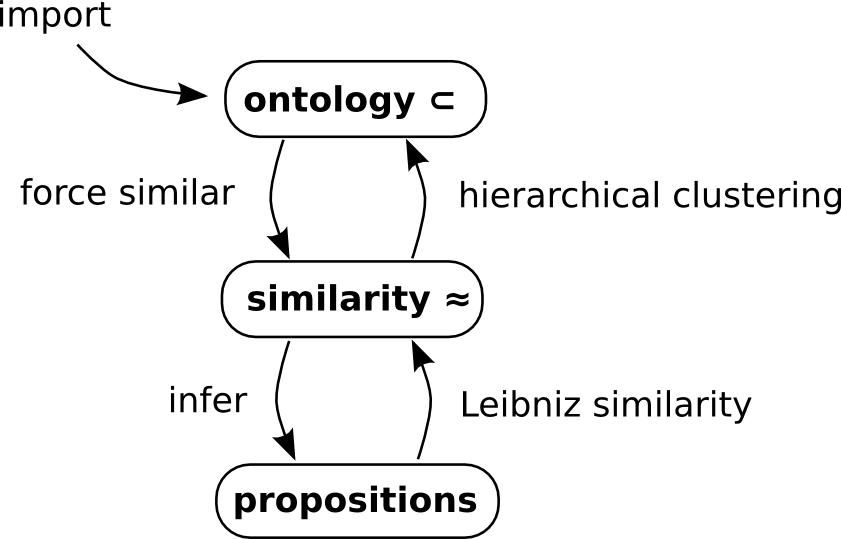
\includegraphics[scale=0.8]{ontology-meta-relations.png}
\end{figure}

我们想把这个结构映射到 Banach 空间。

虽然这个 metric 很难计算,但它可能是我们的学习问题里唯一比较合理的结构,除了用它之外可能没有其他选择。

这个 metric 其实不是良好定义的,因为它可能不会 converge。  举例来说,Reimann hypothesis 原来和质数的分布有关,但这关系在1859年以前人们还不知道。  在逻辑上我们可以推导出很深的关系,这似乎是永无止境的。  但如果我们假设可以得到近似的 metric,这个 heuristic 也许还不错。

\section{Neural Tensor Network}

Andrew Ng 是香港人,Coursera 的 machine learning 教授,他在 Stanford,最近加入了百度。 他和合作者提出了 NTN 模型\cite{Socher2013}:
$$ \top(a\, R\, b) = u^T \; \sigmoid \, (a^T \, U \, b + W {{a}\choose{b}} + c ) $$
$\top(a\, R\, b)$ 表示 $a\, R\, b$ 这个关系的\textbf{强度}。\\
$U$ 是一个 tensor,取两个向量 $a, b$ 给出第三个向量 $a^T \, U \, b$(它服从张量的双线性性质)。\\
$W$ 是一个矩阵,$W {{a}\choose{b}}$ 是一层传统的神经网络,$\sigmoid$ 是一个非线性函数。\\
$u^T$ 是一粒神经元,作用是把各个分量加起来,得出一个数。

\section{Paul Smolensky's tensor representation}

Paul Smolensky 的书是《The harmonic mind》(2006)\cite{Smolensky2006},第一卷是 AI 理论,第二卷是语言学理论。

他提出用张量来表示关系,一般而论:
\begin{eqnarray}
father(john, pete) & \Leftrightarrow & father \otimes john \otimes pete \nonumber \\
Var_1 : val_1, Var_2 : val_2 & \Leftrightarrow & Var_1 \otimes val_1 + Var_2 \otimes val_2 \nonumber 
\end{eqnarray}
第二句的意思是,$variable_1$ 的值是 $value_1$,$variable_2$ 的值是 $value_2$。 

他引入了 ``role'' 和 ``filler'' 的概念:  $variable_i$ 是 role, $value_i$ 是 filler。 用这个方法来做 variable binding,好处是可以避免 $ A \cdot B = B \cdot A $ 的问题。

举例来说,在自然语言中可以有这个 句子结构:
$$ s = \quad \raisebox{-.5\height}{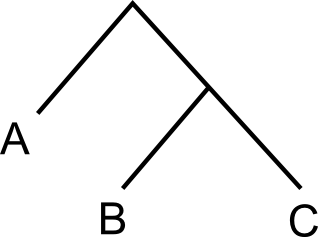
\includegraphics[scale=0.75]{Smolensky-tree.png}} $$

$r_0$ 和 $r_1$ 分别是树的左右孩子的 roles。 用张量积表示:
\begin{eqnarray}
s &=& A \otimes r_0 + q \otimes r_1 \nonumber \\
q &=& B \otimes r_0 + C \otimes r_1 \nonumber \\
\therefore \; s &=& A \otimes r_0 + B \otimes r_0 \otimes r_1 + C \otimes r_1 \otimes r_1 \nonumber
\end{eqnarray}

张量积的好处是, $r_0$ 和 $r_0 \otimes r_1$ 是不同的元素,它们彼此不会「相撞」。  坏处是当乘积的长度增加时,dimension 也增加得很快。 

下表是 Smolensky 表示法的总结:
\begin{center}
\begin{tabular}{|c|c|c|}
\hline
                    & Example & Vector representation \\
\hline
Set element         & $\{ c_1, c_2 \}$ & $ c_1 + c_2 $ \\ 
\hline
Filler-role binding & $ AB = \{ A \backslash r_1, B \backslash r_2\} $ & $ A \otimes r_0 + B \otimes r_1 $\\
\hline
Recursive structure & \raisebox{-.5\height}{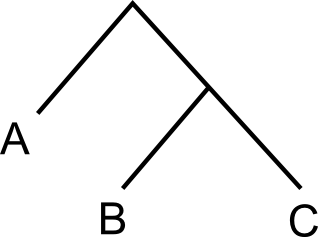
\includegraphics[scale=0.5]{Smolensky-tree.png}} & $A \otimes r_0 + [BC] \otimes r_1$ \\
\hline
\end{tabular}
\end{center}

% 和我的 naive 办法相比,有什么分别?  

我在博客\footnote{\href{http://geniferology.blogspot.hk/2015/03/what-are-tensors.html}{blog post}}上解释过,tensor 是所有 bi-linear forms 的 universal form。 如果有向量空间 $U$ 和 $V$,
\begin{eqnarray}
T: & U \otimes V \rightarrow W \nonumber \\
t: & u \otimes v \mapsto w \nonumber 
\end{eqnarray}
那么在 $U, V$ 中线性无关的 $\{u_1, ..., u_m \}$ 和 $\{ v_1, ..., v_n \}$,它们的乘积 $\{ u_i \otimes v_i \}$ 在 $W$ 中仍然是线性无关的。  这是 tensor product 的一个 defining property,换句话说:
$$ \mbox{线性无关集} \otimes \mbox{线性无关集} \mapsto \mbox{线性无关集} $$
而这正是我们需要的,因为根据「scalar = 逻辑命题真假值」的诠释,这正是命题之间不「相撞」的条件。

Antony Browne \& Ron Sun 的较早的论文《Connectionist inference models, 2001》\cite{Browne2001}有讲述更多 neural-symbolic integration 的做法。

\section{Coecke-Sadrzadeh-Clark representation}

这是 Coecke, Sadrzadeh, Clark (2010)\cite{Coecke2010} 提出的表示法。

它首先是基於 categorial grammar(类型语法),那是一种有「左右除法」的文法,例如在\english{John likes Mary} 这句子中,\english{likes} 的类型是:
$$ likes := (S\backslash NP)/NP $$
意思是当\english{likes} 这个字,在左边乘一个 noun phrase,右边乘另一个 noun phrase,之后便可得到一个句子 S。 这种文法由 Lambek 1958 年开创。

换成 tensor product,\english{likes} 表示成一支 vector:
$$ \overrightarrow{likes} \in N \otimes S \otimes N $$
这是很合理的,因为 这个 tensor product space,它的元素就是那些 multi-linear functions:
$$ f : N \times N \rightarrow S. $$

\section{Metric embedding}

最近有一本新书:[Mikhail Ostrovskii 2013] \textit{Metric embeddings: bi-Lipschitz and coarse embeddings into Banach spaces}\cite{Ostrovskii2013},它似乎正正讲述了我们将 logic 嵌入到「连续空间」的问题。

What is the bi-Lipschitz condition?  A map $f: X \rightarrow Y$ is called a \textit{C-bi-Lipschitz embedding} if there exists $r > 0$ such that
$$ \forall u,v \in X, \;\; r\, d_X(u,v) \leq d_Y(f(u), f(v)) \leq r C\, d_X(u,v) $$
for some $C < \infty$.  The smallest constant $C$ for which there exists $r > 0$ such that the above is satisfied is called the \textit{distortion} of the map $f$.  这似乎定义了「远的保持远、近的保持近」的意思。

\section{SVMs and the kernel trick}

印象中 \textbf{SVM} (support vector machine) 似乎可以将非凸的问题转化成凸优化的问题; 可不可以将这个想法应用到我们的问题上呢?

SVM 的算法,首先用 kernel trick 将 data points 转换到高维空间,然后在高维空间中进行线性的 hyperplane 分割。

所谓 \textbf{kernel trick} 是指: 给定一个 inner product,它暗含了一个到高维空间的转换 $\phi$ (但这个转换不需要真的计出来)。

%A given dot product implicitly defines a transformation $\phi$ into higher dimensional space.  In such a space the data set might be linearly separable.

\begin{figure}[H]
\centering
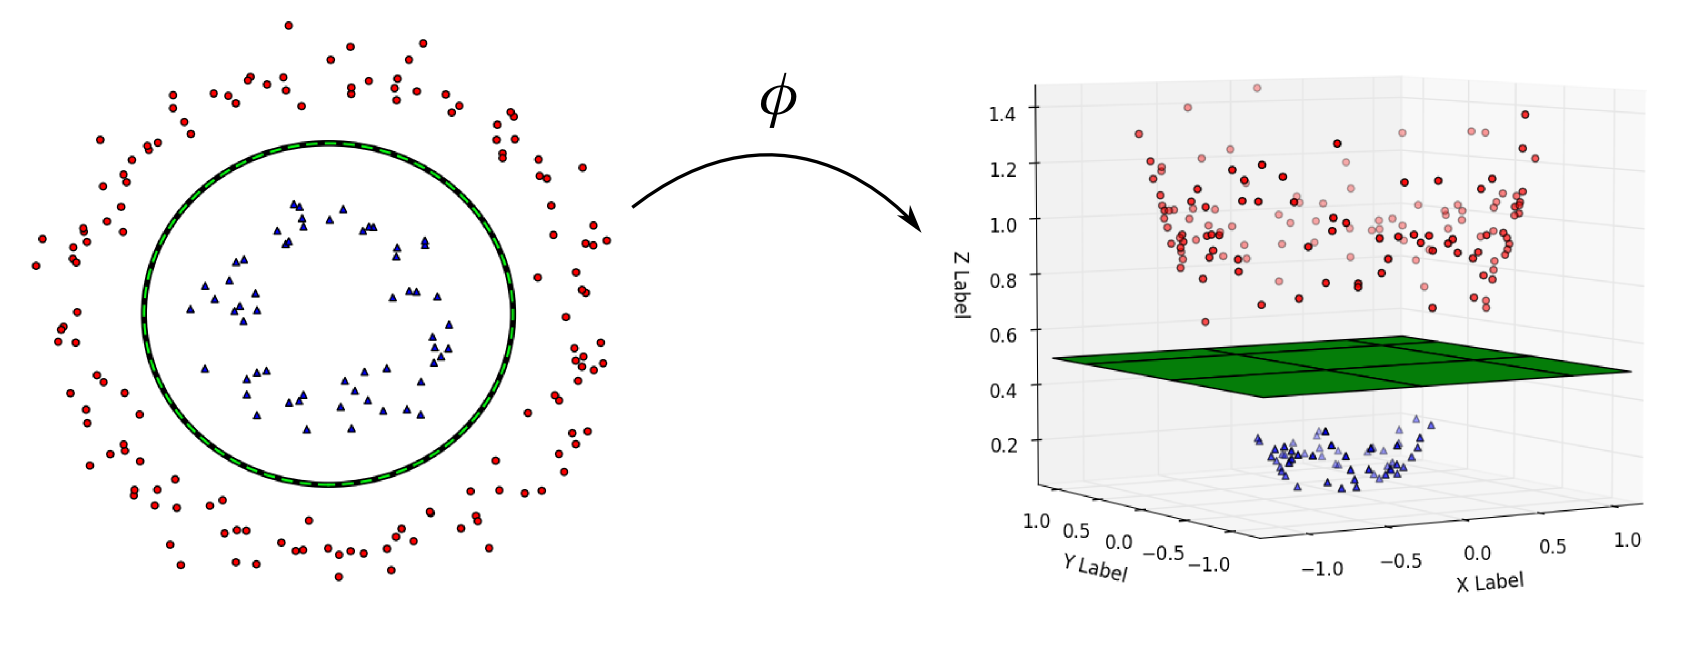
\includegraphics[scale=0.6]{kernel-trick.png}
\end{figure}

而,在高维空间中用线性分割,那 error term 是一些正交距离,所以是 \textbf{quadratic form},所以这问题是\textbf{凸优化}。

%The \textbf{quadratic form} comes from the linear separation, and that's why the problem is a convex optimization problem.

我们的问题是性质不同的,但两者似乎有些相似... 

\section*{Acknowledgments}

最近在香港认识了两个朋友,Dr 陈启良 (CUHK) 和 Dr 譚志斌 (HSMC),和他们谈过我的 AI 理论之后获益良多。

\bibliographystyle{plain} % or number or aaai ...
\bibliography{AGI-book}

% \onecolumn

% Bigger figures

\end{document}
